\subsection{Atari Puffer}
Der 1982 von Atari entwickelte \textit{Atari Puffer} (Abb \ref{ataripuffer}) \cite{Sinclair:2007:CDE:1321261.1321313} war das erste System, welches die Möglichkeit bieten
sollte Videospiele mit dem Körper zu steuern. Plan war es eine Art Fahrradergometer an den \textit{Atari} 					anzuschließen um somit die Spiele zu steuern. Eine erhöhte Umdrehungszahl der Pedale sollte dafür sorgen,
dass zum Beispiel das Auto des Spielers im Spiel \textit{Pole Position} schneller fuhr oder der Spieler im Spiel
\textit{Dig-Dug} schneller gräbt. Zusätzlich konnte ein Gamepad am Lenker montiert werden um zusätzliche
Eingaben zu ermöglichen.\\
Auf Grund der Videospielkrise im Jahr 1984 kam es jedoch nie zur Markteinführung.\\
\begin{figure}[h]
	\centering
	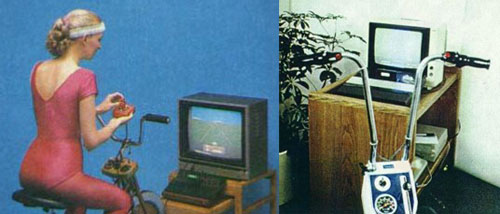
\includegraphics[width=7cm]{gfx/recherche/ataripuffer.jpg} 
		\caption{Atari Puffer}
	\label{ataripuffer}
\end{figure}


\subsection{Thera Trainer}
Die Firma \textit{medica Medizintechnik GmbH} entwickelt, neben dem \textit{Balance-Trainer}, verschiedene Geräte und Programme zur Unterstützung der Bewegungstherapie. Mögliche Anwendungszwecke sind beispielsweise die Therapie von Schlaganfällen, sowie von Muskel- und rheumatischen Erkrankungen. Es findet jedoch auch Anwendung auf dem Gebiet der Orthopädie und Kardiologie. Hierzu bietet der Hersteller verschiedene Trainingsgeräte in Form von Ergometern und Balance Plattformen.\\
\begin{figure}[ht]
	\centering
	\begin{subfigure}{6 cm}
	\centering
			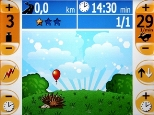
\includegraphics{gfx/recherche/Igel.jpg}
			\caption{Igel}
			\label{Igel}
	\end{subfigure}
	\begin{subfigure}{6 cm}
	\centering
			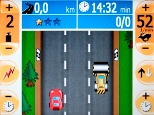
\includegraphics{gfx/recherche/Auto.jpg}  
			\caption{Auto}
			\label{Auto}
	\end{subfigure}
	\caption{Thera Trainer}
\end{figure}\\
Auf dem am Gerät montierten Bildschirm können verschiedene optische Feedbacksysteme angezeigt werden:

\paragraph{Igel:}\noindent
Durch unterschiedliche Kraftverteilung des linken und rechten Beins bewegt sich der Igel in die entsprechende Richtung. Herab fallende Gegenstände sollen dadurch zum platzen gebracht werden. (Abb.~\ref{Igel})

\paragraph{Auto:}\noindent
Der Patient sieht eine Fahrbahn, sowie sein eigenes Fahrzeug. Ziel ist es möglichst viele andere Fahrzeuge zu überholen. Hierzu muss er schneller Treten als eine voreingestellte Drehzahl. Durch Veränderung der Kraftverteilung (siehe \textit{Igel}) kann das Auto nach links und rechts bewegt werden. (Abb.~\ref{Auto})

\subsection{Jeff Sinclaire - Edith Cowan University}
\begin{figure}[ht]
	\centering
	\begin{minipage}[b]{6 cm}
		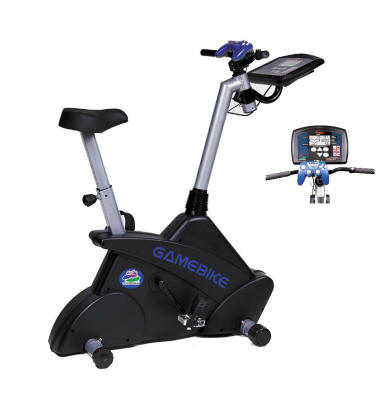
\includegraphics[width=5cm]{gfx/recherche/cateye.jpg} 
			\caption{CatEye GameBike}
			\label{gamebike}
	\end{minipage}
	\begin{minipage}[b]{6 cm}
			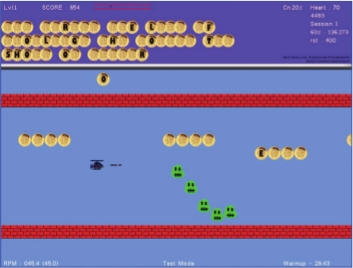
\includegraphics[width=5cm]{gfx/recherche/edith.jpg}  
			\caption{Side Scroller}
			\label{sidescroller}
	\end{minipage}
\end{figure}\noindent
Bei dem Exergaming Projekt der \textit{Edith Cowan University Perth} \cite{5716909} handelt es sich um einen einfachen Side-Scroller, der mit einem Fahrradergometer gesteuert wird (Abb. \ref{sidescroller}). Ziel des Spiels ist es einen Hubschrauber in der richtigen Höhe zu halten und dabei Gegenstände einzusammeln, Hindernissen auszuweichen und Gegner abzuschießen. Je schneller der Spieler tritt, desto höher fliegt der Helikopter. Verringert der Spiele die Geschwindigkeit verliert der Helikopter an Höhe.\\
Als Ergometer kommt hierbei das \textit{GameBike} der Firma \textit{CatEye} (Abb. \ref{gamebike}) zum Einsatz. Das Ergometer kann an die gängigsten, auf dem Markt erhältlichen Spielekonsolen angeschlossen werden und funktioniert mit sämtlichen Spielen, die auf Geschwindigkeit basieren. Für das Projekt der Universität Perth wurde eine Modifikation vorgenommen um es auch an einen PC anschließen zu können.


\subsection{Ergo Active}
Entwickelt wurde \textit{Ergo Active} an der \textit{Technischen Universität Darmstadt} \cite{Gobel:2010:SGH:1873951.1874316} zur Förderung von Serious Games for Health mit wissenschaftlichem Hintergrund, in Bezug auf Sport und Gesundheit. Es umfasst drei Spiele \textit{Taubenjagd, Film} und \textit{Balance} zum Ausdauer-, beziehungsweise Herz-Kreislauftraining. Gesteuert werden alle drei Spiele mittels eines Fahrradergometers.

\paragraph{Taubenjagd:}\noindent
Hierbei handelt es sich um einen einfachen Sidescroller. Der Spieler steuert eine Brieftaube mit Hilfe des Fahrradergometers. Ziel ist es vorbei fliegende Briefe einzusammeln um Punkte zu bekommen. Um so schneller er tritt, desto höher fliegt die Taube. Der Spieler tritt dabei innerhalb eines vorher festgelegten Geschwindigkeit Intervalls, wodurch einerseits verhindert wird, dass der jeweilige Spieler ausserhalb seiner körperlichen Möglichkeiten trainiert und andererseits ein Adaptionsmechanismus für verschiedene Spieler gegeben ist. 

\paragraph{Film:}\noindent
\textit{Film} ermöglicht dem Spieler zum Beispiel Etappen der \textit{Tour de France nachzufahren}. Hierfür wird ein Film der jeweiligen Strecke gezeigt. Je nach dem wie schnell der Spieler Tritt um so schneller wird der Film der jeweiligen Etappe abgespielt. Ähnlich wie bei Taubenjagd findet auch hier eine Überwachung des Spielers statt. Über-, oder unterschreitet er seine Leistungsgrenzen gibt das Spiel ein Signal um den Spieler daraufhin zuweisen wieder innerhalb seines persönlichen Intervalls zu trainieren.

\paragraph{Balance:}\noindent
Bei \textit{Balance} hat der Spieler zwei Aufgaben. Er balanciert einen Clown auf einem Ball. Hierzu muss er mittels Ergometer eine vorgegebene Geschwindigkeit halten, beziehungsweise darf maximal nur um einen bestimmten Wert davon abweichen. Während er den Clown in der Balance hält fallen Luftballons herab, die er mittels Maus oder Wiimote abschießen muss, um Punkte zu sammeln. Die voreingestellte Geschwindikeit und die maximale Abweichung dienen hierbei zur Überwachung, damit  sich der Spieler innerhalb seiner Leistungsgrenzen bewegt. 
\begin{figure}[ht]
	\centering
	\begin{minipage}[b]{6 cm}
			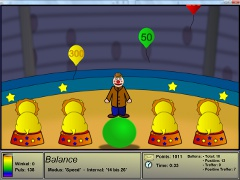
\includegraphics[width=6cm]{gfx/recherche/balance.jpg} 
			\caption{Ergo Active - Balance}
			\label{balance}
	\end{minipage}
	\begin{minipage}[b]{6 cm}
			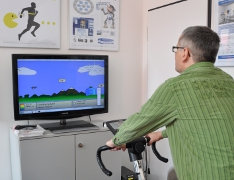
\includegraphics[width=6cm]{gfx/recherche/ergoactive.jpg} 
			\caption{Taubenjagd}
			\label{ergoactive}
	\end{minipage}
\end{figure}

\section{Fazit der Recherche}
In Bezug auf die benutzte Hardware von anderen Systemen, erkennt man, dass Fahrradergometer sehr oft als das bevorzugte Mittel zur Eingabe genutzt werden. Fahrradergometer bieten jedoch nur eine sehr limitierte Bandbreite von möglichen Eingaben. Streng genommen findet man in den betrachteten Systemen ausschließlich zwei Aktionen, die Erhöhung der Trittfrequenz, sowie die Verringerung, beziehungsweise Abbremsen um eine Spielfigur zu steuern und Aktionen einzuleiten \\
Auch in Bezug auf die beanspruchten Körperpartien werden stets nur der untere Teil des Körpers, speziell die Beine, belastet. Einzige Ausnahme sind die Produkte der Firma \textit{medica Medizintechnik GmbH}. Sie bieten ebenfalls Ergometer die mit der Hand und den Armen bedient werden können und sind somit auch, zum Beispiel, für Rollstuhlfahrer geeignet. Alle Systeme jedoch benutzen jeweils nur einen Teil des Körpers zur Eingabe - entweder Beine oder Oberkörper. Keines der betrachteten Systeme bietet die Möglichkeit sowohl Ober- als auch Unterkörper zu aktivieren. \\
Kaum ein System bietet neben der Trittfrequenz, beziehungsweise Geschwindigkeit des Ergometers weitere Eingabeoptionen. Das in unserem Projekt genutzte Ergometer bietet diese Möglichkeit jedoch. Durch die Gewichtsverlagerung mit Hilfe des Oberkörpers können wir in unserem Spiel eine weitere Ebene der Kontrollmöglichkeiten erreichen. Hierdurch wird ermöglicht, dass sich die Spielfigur in diesem Projekt in zwei, statt wie in den anderen Publikationen, nur in einer Dimensionen bewegen kann. Darüber hinaus soll in diesem Projekt eine weitere, dritte Dimension, der Bewegungsfreiheit, das Springen, eingebaut werden. Durch die verschiedenen Aspekte der Steuerung soll die Motivation des Spielers möglichst hoch gehalten werden, da das Spiel vielfältiger ist. Andere Projekte beschränken sich lediglich auf eine mögliche Eingabe, wodurch die Gefahr entsteht, dass das Spiel schnell eintönig und langweilig wird.\\
Trotz der Erweiterten Eingabemöglichkeit dieses Systems im Vergleich zu anderen Projekten, besitzt sie dennoch nicht die volle Bandbreite der möglichen Kommandos, wie es zum Beispiel Spiele bieten, die an einem Stationären Computer mit Tastatur und Maus gesteuert werden. Aus diesem Grund muss das entwickelte Spiel ebenfalls eine einfache, aber interessante, Spielmechanik mit hohem Motivationsfaktor haben. Die beiden betrachteten Spiele \textit{Skyroads} und \textit{Audiosurf} sind hierfür gute Beispiele. Sie kommen jeweils mit verhältnismäßig wenigen Eingaben aus, bieten jedoch trotzdem eine attraktive und motivierende Spielmechanik. Aus diesem Grund sollen diese beiden Spiele eine Art Vorbild für das im Rahmen dieses Praktikums entwickelten Bewegungsspiels darstellen. Ziel wird es sein interessante Konzepte zu Adaptieren, beziehungsweise zu erweitern um die Funktionen des Fahrradergometers möglichst optimal nutzen zu können.
